\documentclass[tikz]{standalone}
\usetikzlibrary {arrows.meta, shapes.geometric}

\begin{document}
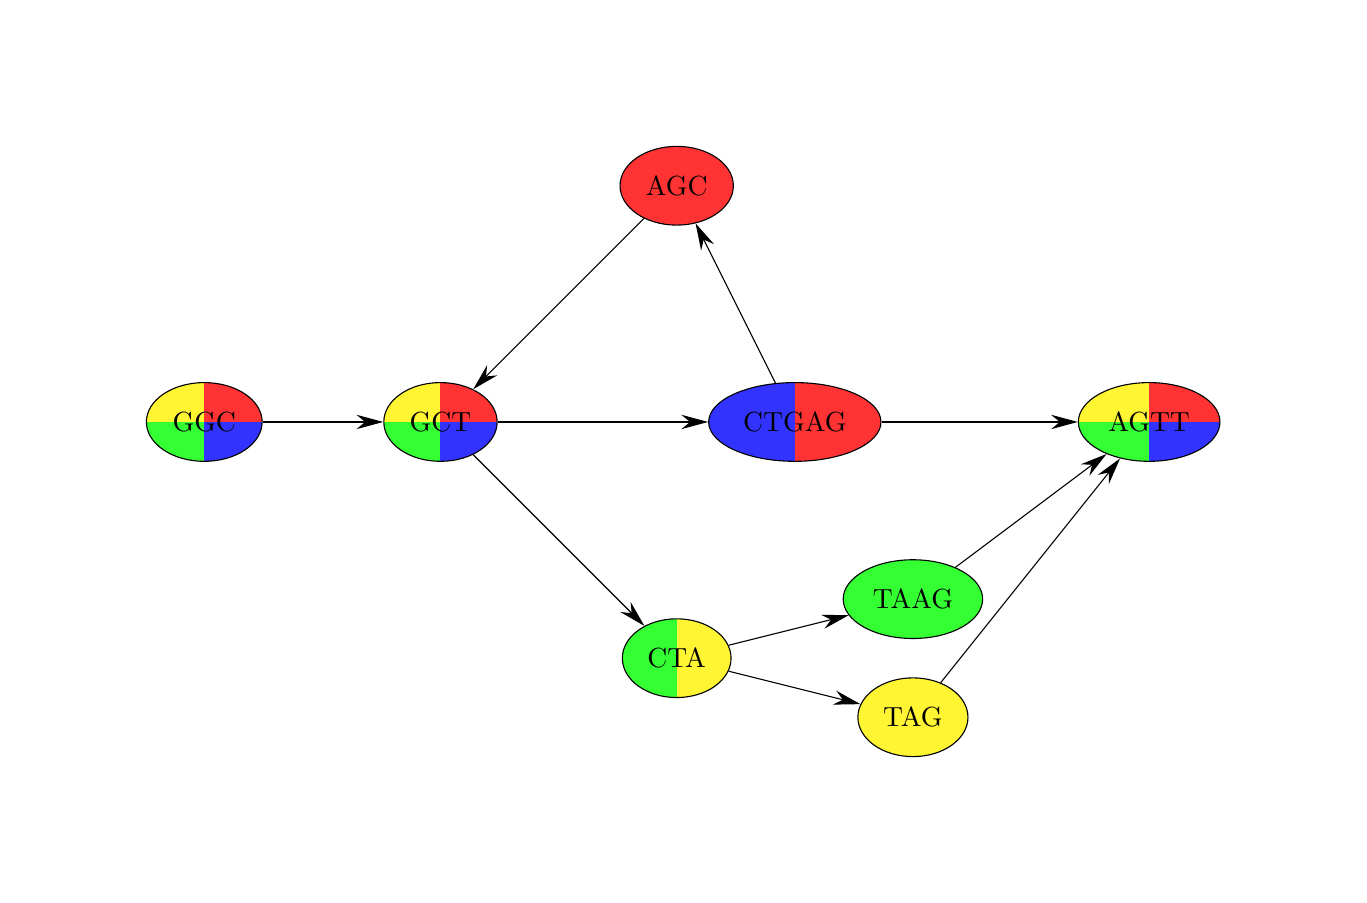
\begin{tikzpicture}[scale=1.5,
                        every node/.style={ellipse, draw, minimum size=1cm},
                        every path/.style={-{Stealth[length=3mm, angle=30:10pt]}},
                        execute at end picture={\path (current bounding box.south west) +(-1,-1) (current bounding box.north east) +(1,1);} % add margin arround the picture
                    ]

    % Define custom style for varius color fills
    \tikzset{
        one color/.style={
            path picture={
                \fill[#1, opacity=0.8] (path picture bounding box.south west) rectangle (path picture bounding box.north east);           }
        }
    }
    \tikzset{
        two colors/.style n args={2}{
            path picture={
                \fill[#1, opacity=0.8] (path picture bounding box.south west) rectangle (path picture bounding box.north);
                \fill[#2, opacity=0.8] (path picture bounding box.south east) rectangle (path picture bounding box.north);
            }
        }
    }
    \tikzset{   % might look messy for non round nodes
        three colors/.style n args={3}{
            path picture={
                \fill[#1, opacity=0.8] (path picture bounding box.south west) rectangle (path picture bounding box.north east);
                \fill[#2, opacity=0.8] (path picture bounding box.north) -- (path picture bounding box.center) -- (-30:2) arc (-30:90:2) -- cycle;
                \fill[#3, opacity=0.8] (path picture bounding box.north) -- (path picture bounding box.center) -- (-120:2) arc (210:90:2) -- cycle;
            }
        }
    }
    \tikzset{
        four colors/.style n args={4}{
            path picture={
                \fill[#1, opacity=0.8] (path picture bounding box.south) rectangle (path picture bounding box.east);
                \fill[#2, opacity=0.8] (path picture bounding box.south) rectangle (path picture bounding box.west);
                \fill[#3, opacity=0.8] (path picture bounding box.north) rectangle (path picture bounding box.west);
                \fill[#4, opacity=0.8] (path picture bounding box.north) rectangle (path picture bounding box.east);
            }
        }
    }


    % First row of nodes
    \node[one color=red] (A1) at (2, 2) {AGC};

    % Second row of nodes
    \node[four colors={blue}{green}{yellow}{red}] (B0) at (-2, 0) {GGC};
    \node[four colors={blue}{green}{yellow}{red}] (B1) at (0, 0) {GCT};
    \node[two colors={blue}{red}] (B2) at (3, 0) {CTGAG};
    \node[four colors={blue}{green}{yellow}{red}] (B3) at (6, 0) {AGTT};

    % Third row of nodes
    \node (C1)[two colors={green}{yellow}] at (2, -2) {CTA};
    \node (C2)[one color={green}] at (4, -1.5) {TAAG};

    % Fourth row of nodes
    \node (D1)[one color={yellow}] at (4, -2.5) {TAG};

    % Edges between nodes
    \foreach \i in {0,1,2} {
        \pgfmathtruncatemacro{\iplusone}{\i+1}
        \draw (B\i) -- (B\iplusone);
    }
    \draw (A1) -- (B1);
    \draw (B2) -- (A1);

    \draw (B1) -- (C1);
    \draw (C1) -- (C2);
    \draw (C2) -- (B3);

    \draw (C1) -- (D1);
    \draw (D1) to (B3);

    
\end{tikzpicture}
\end{document}